\documentclass[12pt]{article}
\usepackage{graphicx}
\usepackage{hyperref}
\usepackage{amsmath}
\usepackage{amssymb}
\usepackage{siunitx}
\usepackage[numbers, square, sort&compress]{natbib}


\title{Chapter 4: Handling Biomacromolecular Structures for Molecular Docking}
\author{Elvis Martis}
\date{}

\begin{document}

\maketitle

\section{Introduction}

The questions we ask here are, why does the structure and its quality matter? How to check and validate its quality and correctness? And what are consistent and reliable metrics to depend on?  In many computational pipelines, structural models and their quality dictate the outcome and its accuracy. If the structure is wrong, poorly validated, or misinterpreted, such as wrong oligomeric state, mis-modelled ligand, missing loops, the entire workflow can be driven by artefacts rather than biology. Macromolecular structures in public databases, such as the Protein Data Bank (PDB), are not direct experimental observables; they are models derived from experimental data, and the knowledge of chemistry and physics\cite{CH4_Berman2000_PDB,CH4_wwpdb2019protein,CH4_karplus2012linking}.
X-ray crystallography, single-particle cryo-electron microscopy (cryo-EM), and nuclear magnetic resonance (NMR) spectroscopy each provide different types and resolutions of structural information\cite{CH4_Evans2013_data_quality,CH4_Wang2015_structure_quality,CH4_Ulrich2008_BMRB}. Of course, each methodology has its own advantages and disadvantages. Some are resolved using modern computational software packages, while others warrant new experiments. Recently, deep learning-based methods such as AlphaFold have produced highly quality predicted models for large part of the proteome. However, these too have noticeable limitations\cite{CH4_Jumper2021_AlphaFold,CH4_Varadi2022_AlphaFoldDB}, in addition to caveats of the large language models (LLM), such as hallucination of structural features or secondary structural elements that may not be true. 

\begin{figure}[hbt!]
    \centering

    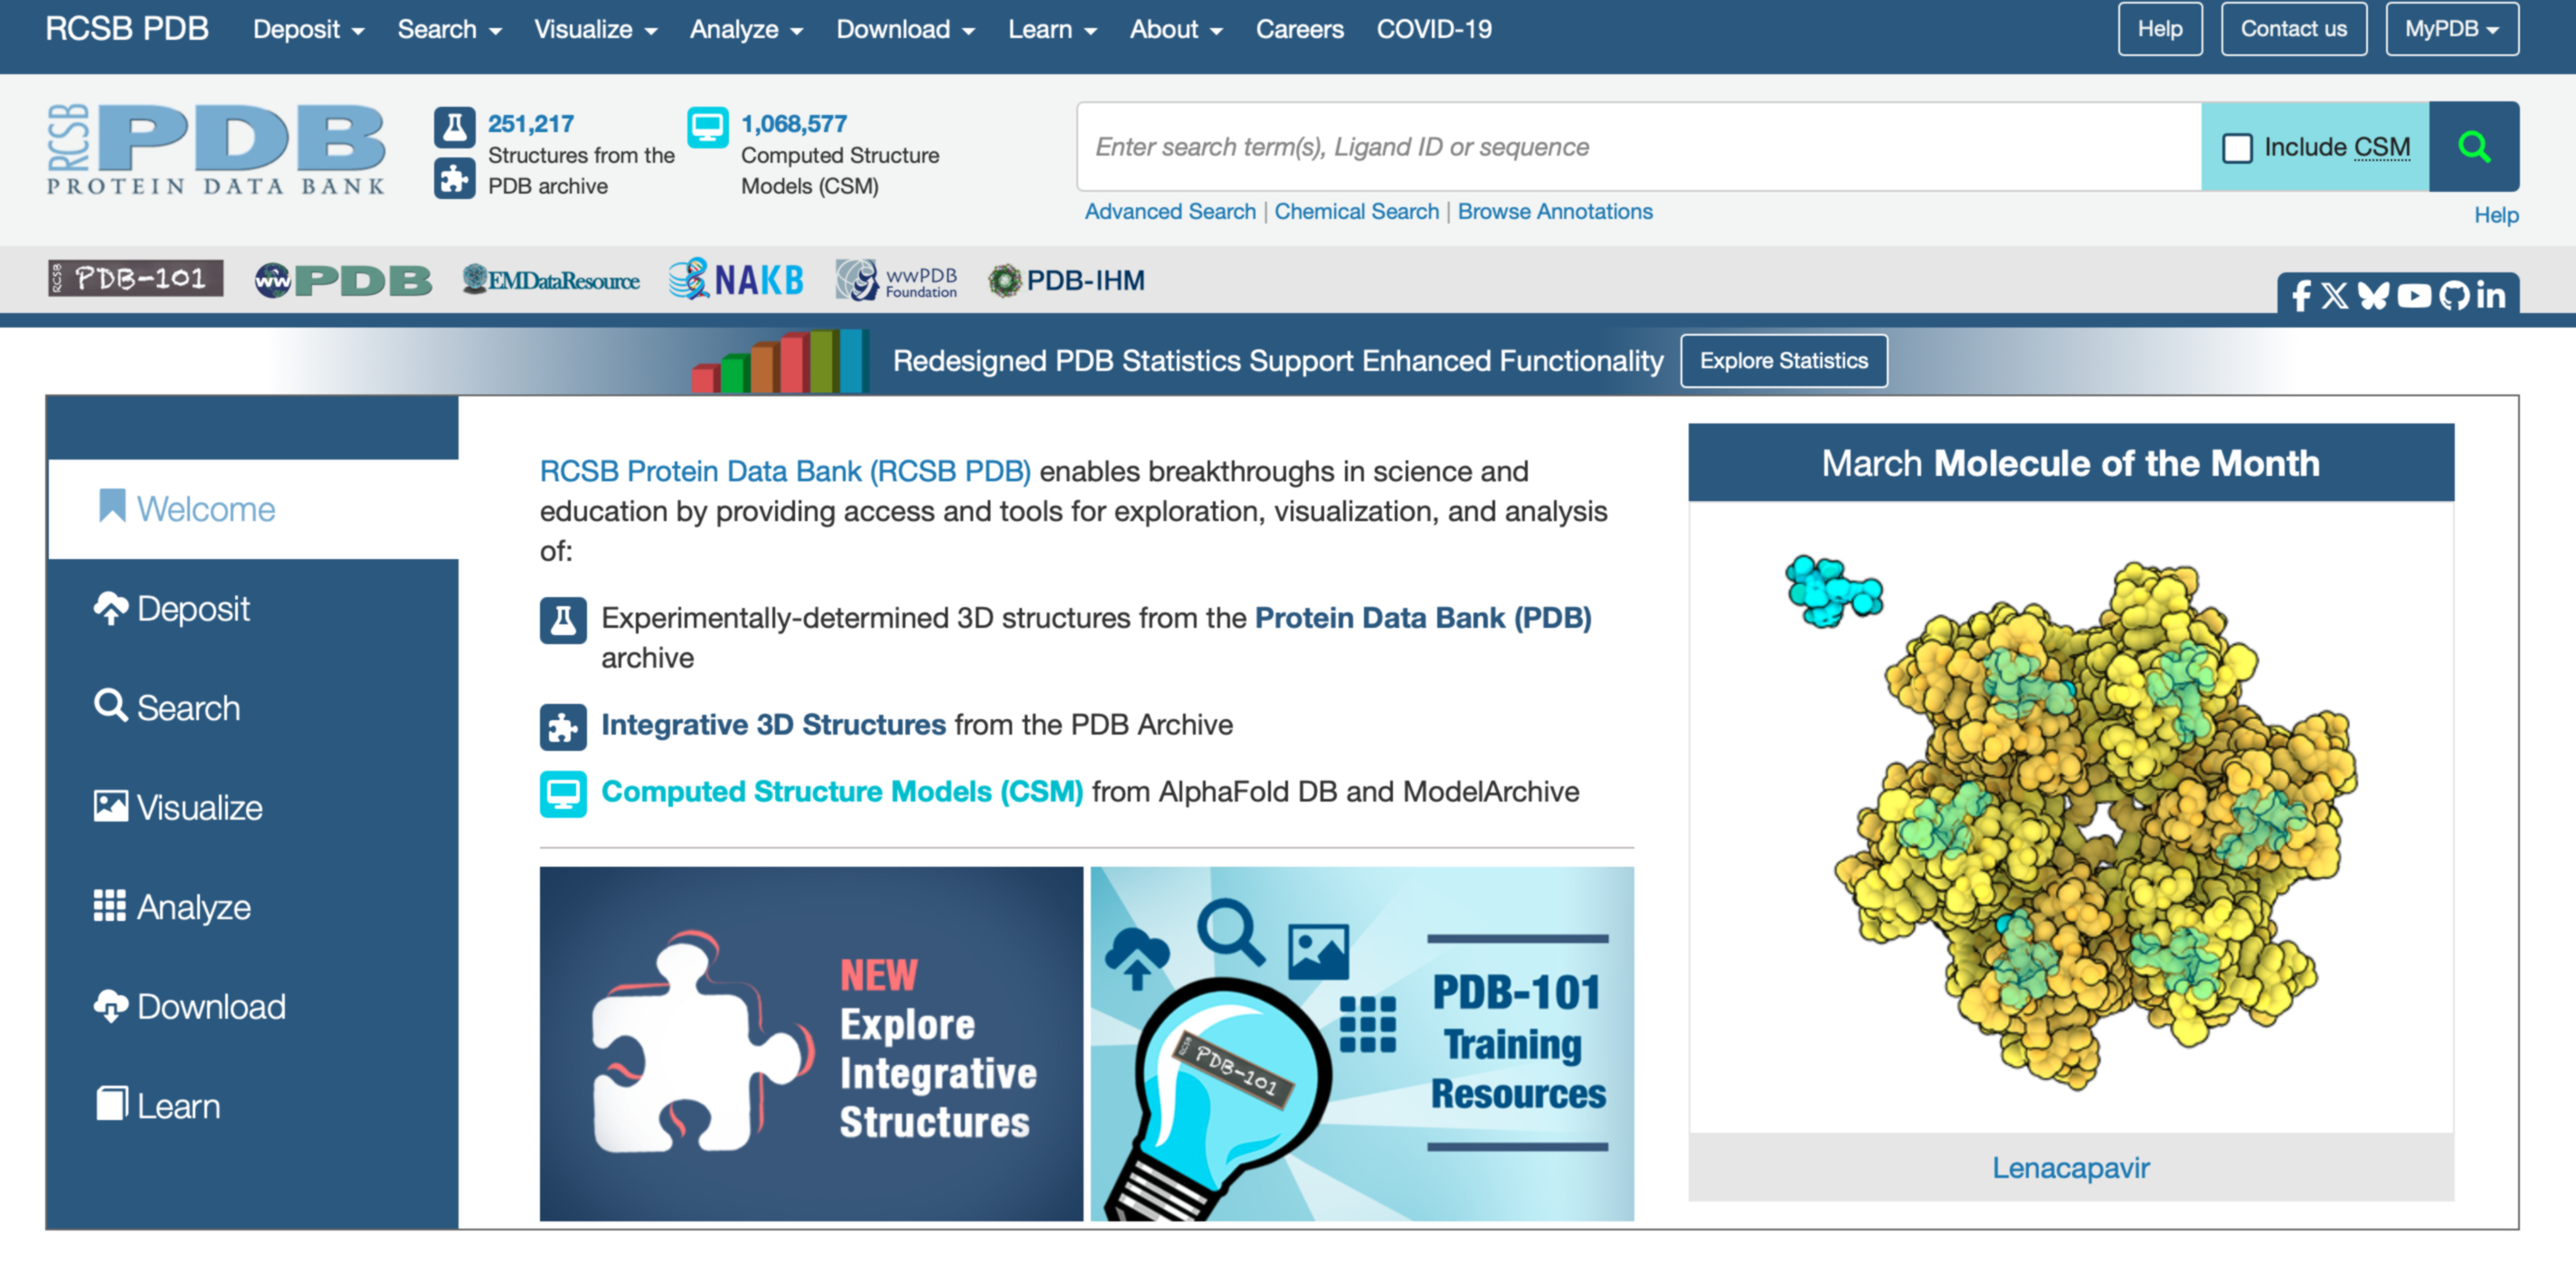
\includegraphics[width=1\textwidth]{RCSB_webpage.jpg}

    \caption{The RCSB Protein Data Bank (PDB) homepage highlighting navigation options to deposit, search, visualize, and analyze  experimentally determined and computed 3D structures} 
\label{fig:RCSBwebpage}
\end{figure}

In this chapter, we aim to introduce the nuances of biomacromolecular models: how they are determined, how to retrieve them from appropriate databases (\textbf{Figure \ref{fig:RCSBwebpage}}), how to interpret their validation metrics, and how to identify and correct docking-related issues. We assume no prior experience in X-ray crystallography, cryo-EM, or NMR. Mathematical details of structure determination and refinement are omitted in favour of conceptual understanding directly relevant to docking.

The emphasis is on the following practical questions
\begin{itemize}
  \item Which resolution and crystallographic quality metrics should be checked, and how to interpret them?
  \item How should missing residues and loops be identified and handled?
  \item How can one distinguish crystal packing multimers from biological assemblies?
  \item What do B-factors really tell us about dynamics, and what are their limitations?
  \item How should post-translational modifications (PTMs) and non-standard residues be treated?
  \item How can ligand and cofactor binding sites and geometries be validated?
  \item How can crystallisation artefacts and crystal environment effects be recognised?
  \item How should electron density maps and cryo-EM maps be used to judge local model quality?
  \item When should updated models from PDB-REDO or predicted models from AlphaFold be preferred?
  \item How can one validate the chosen template structure against complementary data?
\end{itemize}

\section{Experimental Methods}



\subsection{X-ray Crystallography}


Macromolecular X-ray crystallography infers atomic models of biomolecules from X-ray diffraction patterns scattered by crystals.\cite{CH4_Evans2013_data_quality,CH4_Wang2015_structure_quality} A crystal is an ordered array of unit cells, each containing one or more copies of the macromolecule arranged by crystallographic symmetry. The measured diffraction intensities are related to the electron density in the unit cell via a Fourier transform (\textbf{Figure \ref{fig:densitymap}}).  From this density, atomic coordinates are built and refined. X-ray crystallography still accounts for the majority of entries in the PDB.\cite{CH4_Berman2000_PDB,CH4_wwpdb2019protein}

The output from X-ray crystallography relevant to docking are the atomic coordinates, depposited in PDB or mmCIF format for protein, nucleic acids, ligands, cofactors, solvent, and ions. It also gives us structure factors in MTZ or mmCIF format, that contains diffraction amplitudes and, in some cases, phases or anomalous differences. The metadata describe the experimental conditions and global quality metrics such as esolution, R-factors, and completeness

\begin{figure}[hbt!]
    \centering
    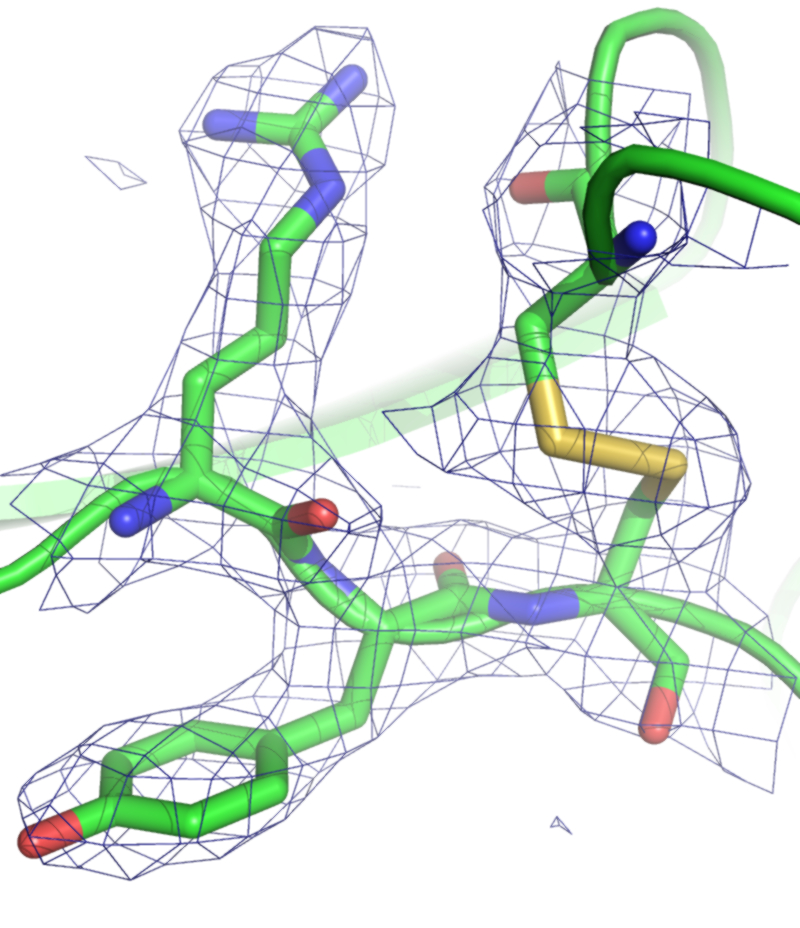
\includegraphics[width=0.7\textwidth]{Density_map.jpg}

    \caption{An example of electron density contoured at 1 $\sigma$, of a crystal structure solved to 2.7 \r{A} resolution. An Arginine residue (top left), a tyrosine residue (bottom left) and a disulphide bond (right) are highlighted. The image is reproduced from \url{https://commons.wikimedia.org/wiki/File:Example_of_electron_density_map.png} under the Creative Commons Attribution-Share Alike 3.0 Unported license.} 
\label{fig:densitymap}
\end{figure}

\subsubsection{Global Quality Indicators}
Crystallographic metrics that are important to assess the quality of the structure is reported in PDB entries and wwPDB validation reports\cite{CH4_Evans2013_data_quality,CH4_Wang2015_structure_quality,CH4_karplus2012linking,CH4_shao2017multivariate}. They include the Resolution (\r{A}), which indicates the highest spatial frequency reliably observed in the diffraction data. At resolutions better than about 2.5\r{A}, side-chain conformations and ligand poses are  well determined. However, the resolution 3--4 \r{A} or worse it becomes difficult to accurately place the side-chain and ligand atoms with confidence. The $\textrm{R}_\textrm{work}$ and $\textrm{R}_\textrm{free}$ measures the agreement between observed and calculated structure factor amplitudes. The $\textrm{R}_\textrm{free}$ is computed using a small subset of reflections excluded from refinement and is a robust indicator of overfitting.\cite{CH4_Wang2015_structure_quality,CH4_karplus2012linking} Typically, a well-refined structures shows  $\textrm{R}_\textrm{free} - \textrm{R}_\textrm{work}$ $\approx$ 0.02--0.05 at medium to high resolution. Furthermore, the data quality metrics, such as completeness, multiplicity, mean intensity over noise $\textrm{I}/\sigma(\textrm{I})$ and correlation coefficient $\textrm{CC}_{1/2}$ between symmetry-equivalent intensities\cite{CH4_Evans2013_data_quality,CH4_Read2011_CC12}.

Here, we would like to emphasis that the resolution alone is not a sufficient measure of quality. Analyses of PDB structures have shown that high-resolution entries can still contain significant model errors, especially in ligand geometries and solvent models.\cite{CH4_shao2017multivariate,CH4_chakraborti2021all}

\subsubsection{Caveats Relevant to Docking}
For SBDD, the caveats mean that one must examine not only global metrics but also local validation around the binding site, including fit to density and the validity of protein-ligand interactions.
Several crystallography-specific factors affect the reliability of the structure for docking. Crystal packing can lead to stabilisation of loop conformations or terminal regions that are weakly populated or absent in solution\cite{CH4_Joosten2009_PDB_related_databanks,CH4_Krissinel2007_PISA}.  Most crystals are measured at cryogenic temperatures to avoid structural damage due to electron bombardment.  This can lead to freezing, which is likely to induce artefacts that can slightly distort structures or redistribute conformational populations. Flexible loops and ligands may be modelled with high $\beta$-factors, partial occupancy, alternate conformations, or omitted altogether. Crystallisation buffers, salts, precipitants, and additives, such polyethene glycols, organic solvents, can bind to the protein and stabilise non-native conformations or oligomeric states. The starting models for molecular replacements, and strong refinement restraints can bias the electron density map towards an incorrect conformation if the data are ambiguous.\cite{CH4_karplus2012linking,CH4_Emsley2010_Coot}


\subsection{Single Particle Cryo-Electron Microscopy}

Single particle cryo-EM reconstructs 3D maps(\textbf{Figure \ref{fig:cryoEMmap}}) of the Coulomb potential from 2D projection images of vitrified biomolecular particles. Individual particle images are aligned and classified, and a 3D reconstruction is computed. Models are then fitted and refined into these maps. The Electron Microscopy Data Bank (EMDB)\cite{CH4_wwpdb2024emdb} is the global archive of 3D CryoEM maps, which are often linked to atomic models deposited in the PDB. An entry in the EMDB that one can download contains the atomic coordinates in PDB/mmCIF file format. The cryo-EM maps and the associated metadata can imported in the MRC/CCP4 format. And lastly, the validation reports, including global and local resolution estimates, and map--model fit metric, can also be obtained.\cite{CH4_pintilie2021validation,CH4_Iudin2016_EM_validation}

\begin{figure}[hbt!]
    \centering
    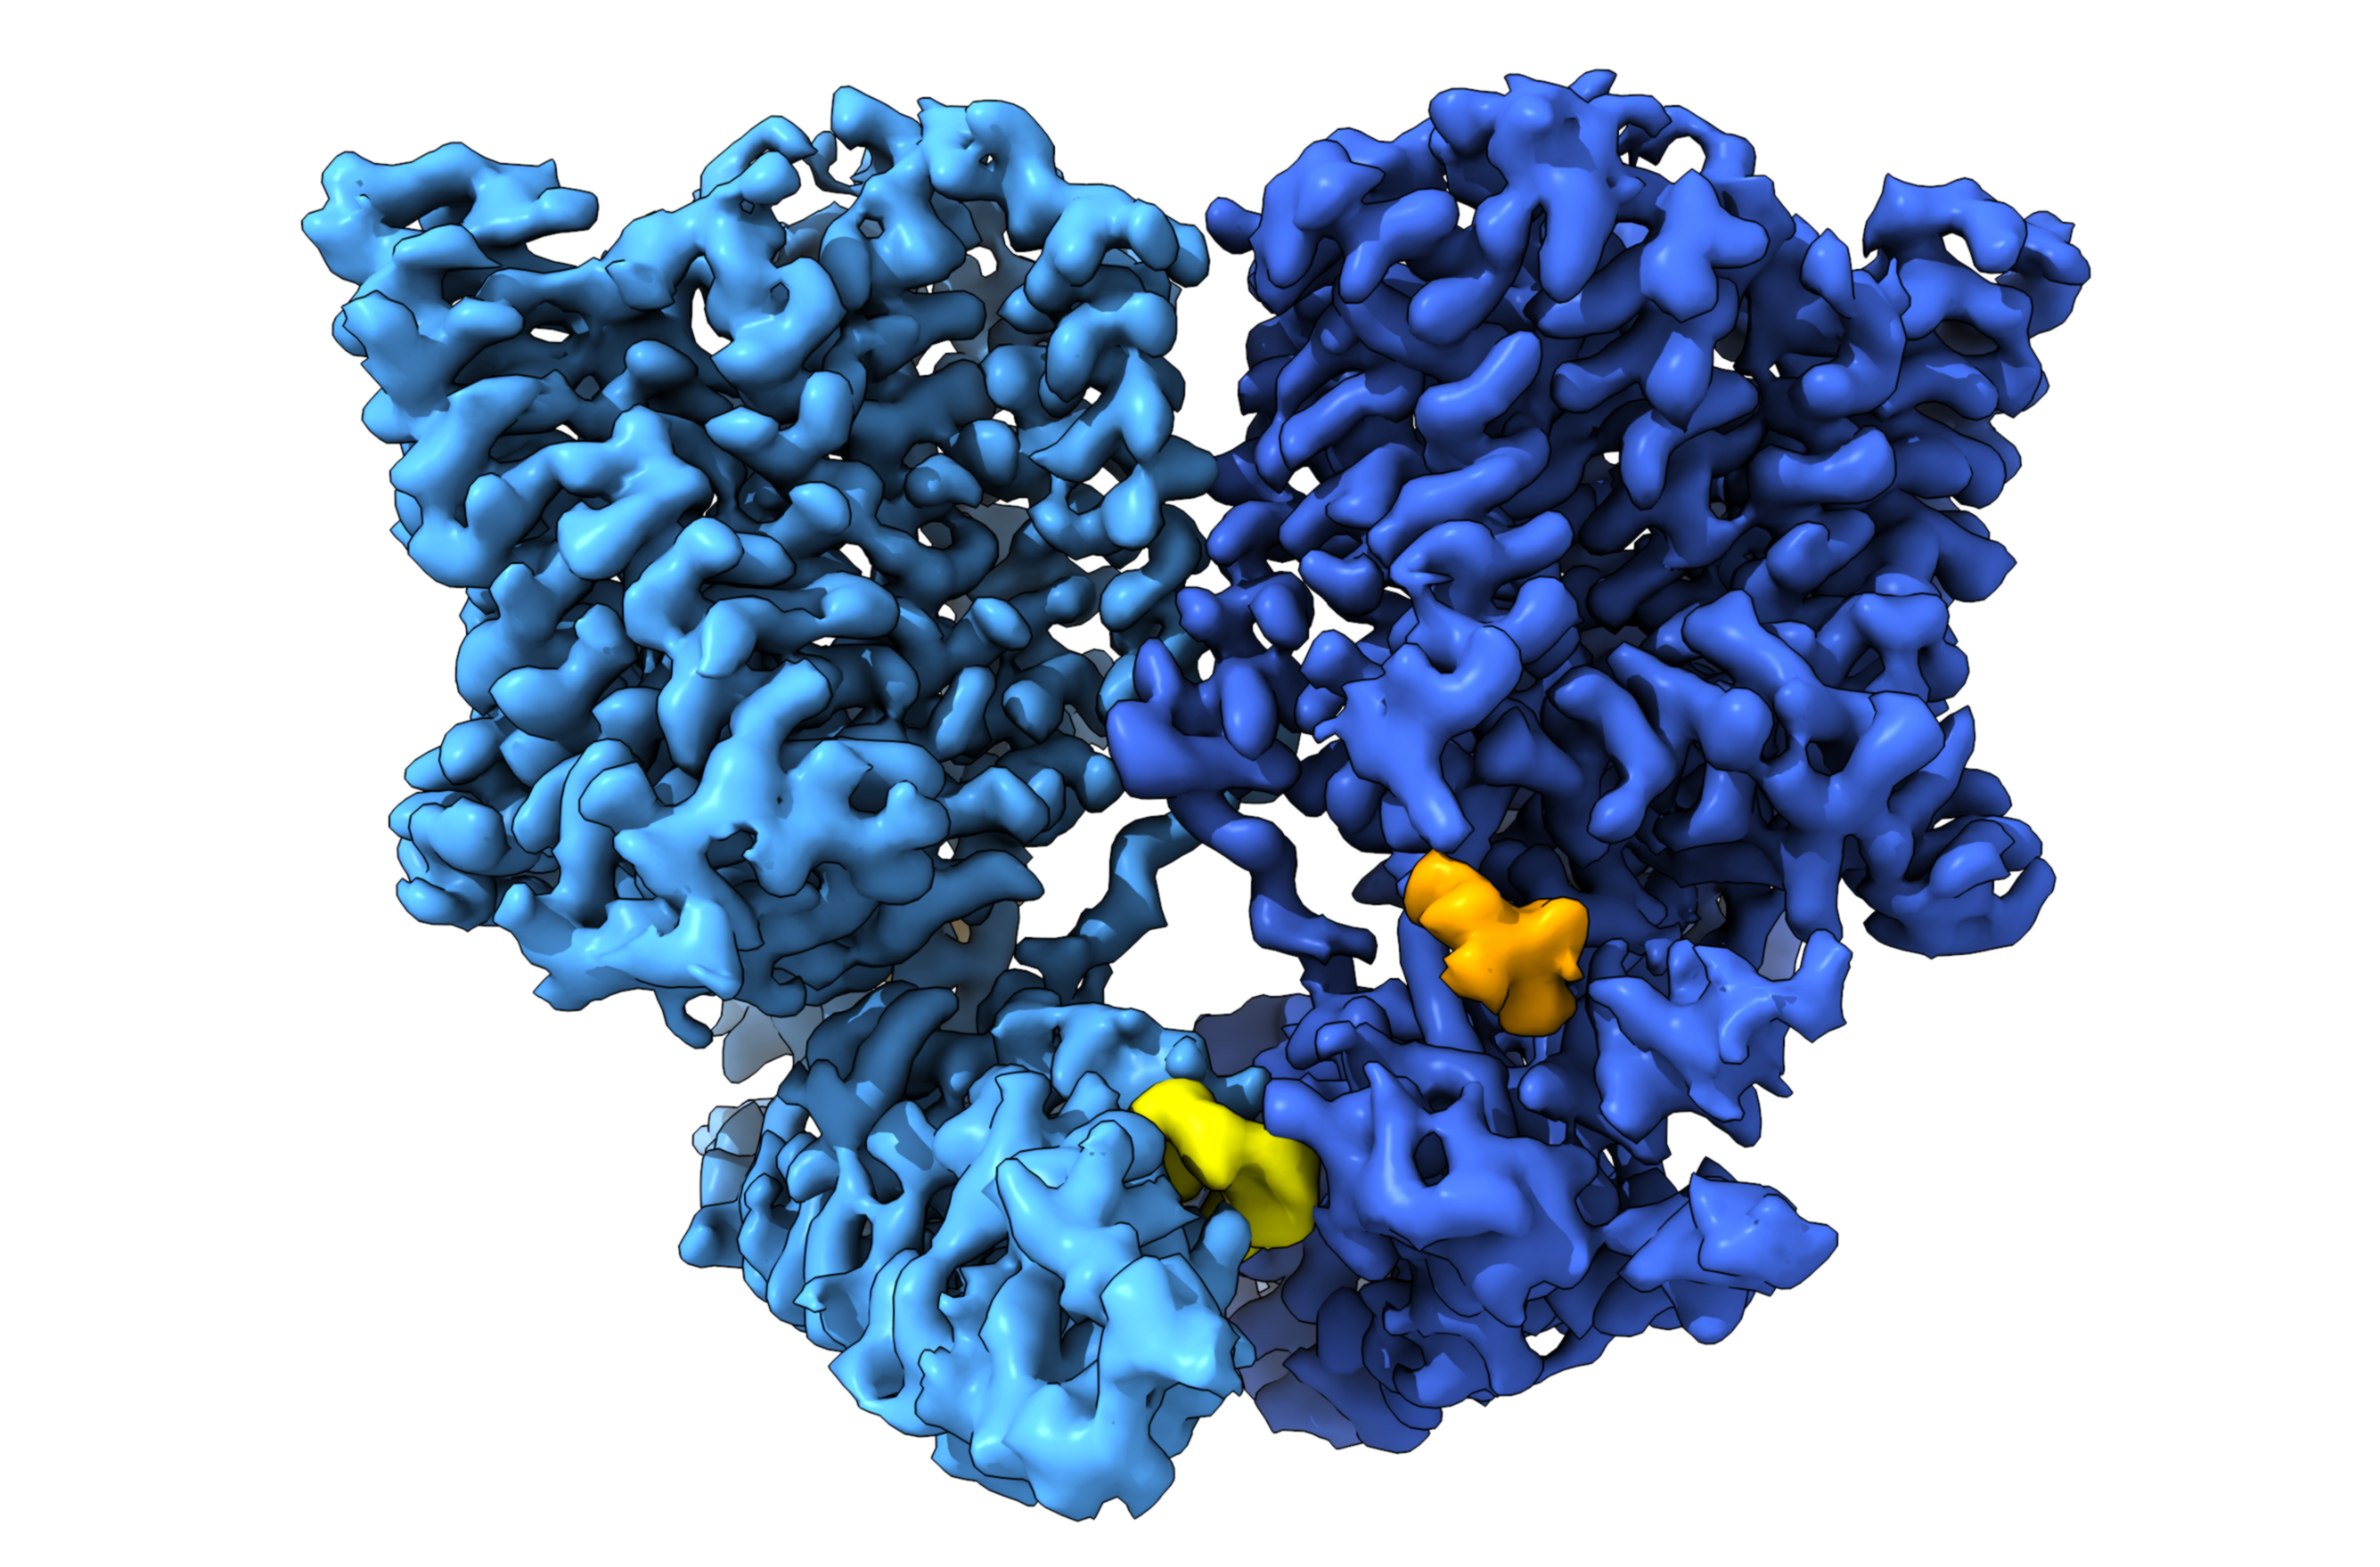
\includegraphics[width=1\textwidth]{cryoEM_map.jpg}
    \caption{The Dimeric human XPR1 was shown as a cyan and blue map, with the InsP7 bound colored in yellow and orange. The image is reproduced from \url{https://commons.wikimedia.org/wiki/File:Human_XPR1_in_complex_with_InsP7.png} under the Creative Commons Attribution 4.0 International license.} 
\label{fig:cryoEMmap}
\end{figure}

\subsubsection{Resolution and Validation}
Cryo-EM uses the Fourier shell correlation (FSC) between independent half-maps to define a global resolution, often reported at the FSC=0.143 threshold\cite{CH4_pintilie2021validation}. However, the map quality is typically heterogeneous, such that the regions of high local resolution co-exist with flexible or disordered regions of much lower resolution. Recent methods, such as FSC-Q and Q-scores\cite{CH4_Pintilie2020_Qscore,CH4_pintilie2021validation}, quantify local map-to-model agreement and highlight regions where the model may be overfitted to noise or under-supported by the data.

Modern validation provides the following data:
\begin{itemize}
  \item Global FSC curves and overall resolution estimates.
  \item Local resolution maps, estimating resolution per voxel or region.
  \item Real space correlation coefficients between map and model, both globally and per residue.
  \item Model geometry statistics, such as, Ramachandran plots, rotamer outliers, clashes, similar to crystallography\cite{CH4_Williams2018_MolProbity}.
\end{itemize}

\subsubsection{Caveats Relevant to Docking}
The global resolution can be misleading, such that the nominal overall resolution may not reflect local resolution in the binding site. This can lead to side chains and ligands that are poorly resolved even at comparatively good nominal resolutions. In some cases multiple conformational states may be averaged, leading to smeared density and ambiguous side-chain or loop positions. The sharpening procedures intended to enhance high-resolution can generate artefactual density features or exaggerate noise, which may lead to overfitting of ligands or side chains. The use of tight masks in refinement can inflate FSC estimates and obscure the true extent of model overfitting. As with X-ray crystallography, proton positions and protonation states are not directly resolved.
Therefore, we strongly recommend thoroughly examining local map quality and map--model correlation in the binding site, rather than relying solely on global nominal resolution. 

\subsection{Solution NMR Spectroscopy}

\begin{figure}[hbt!]
    \centering
    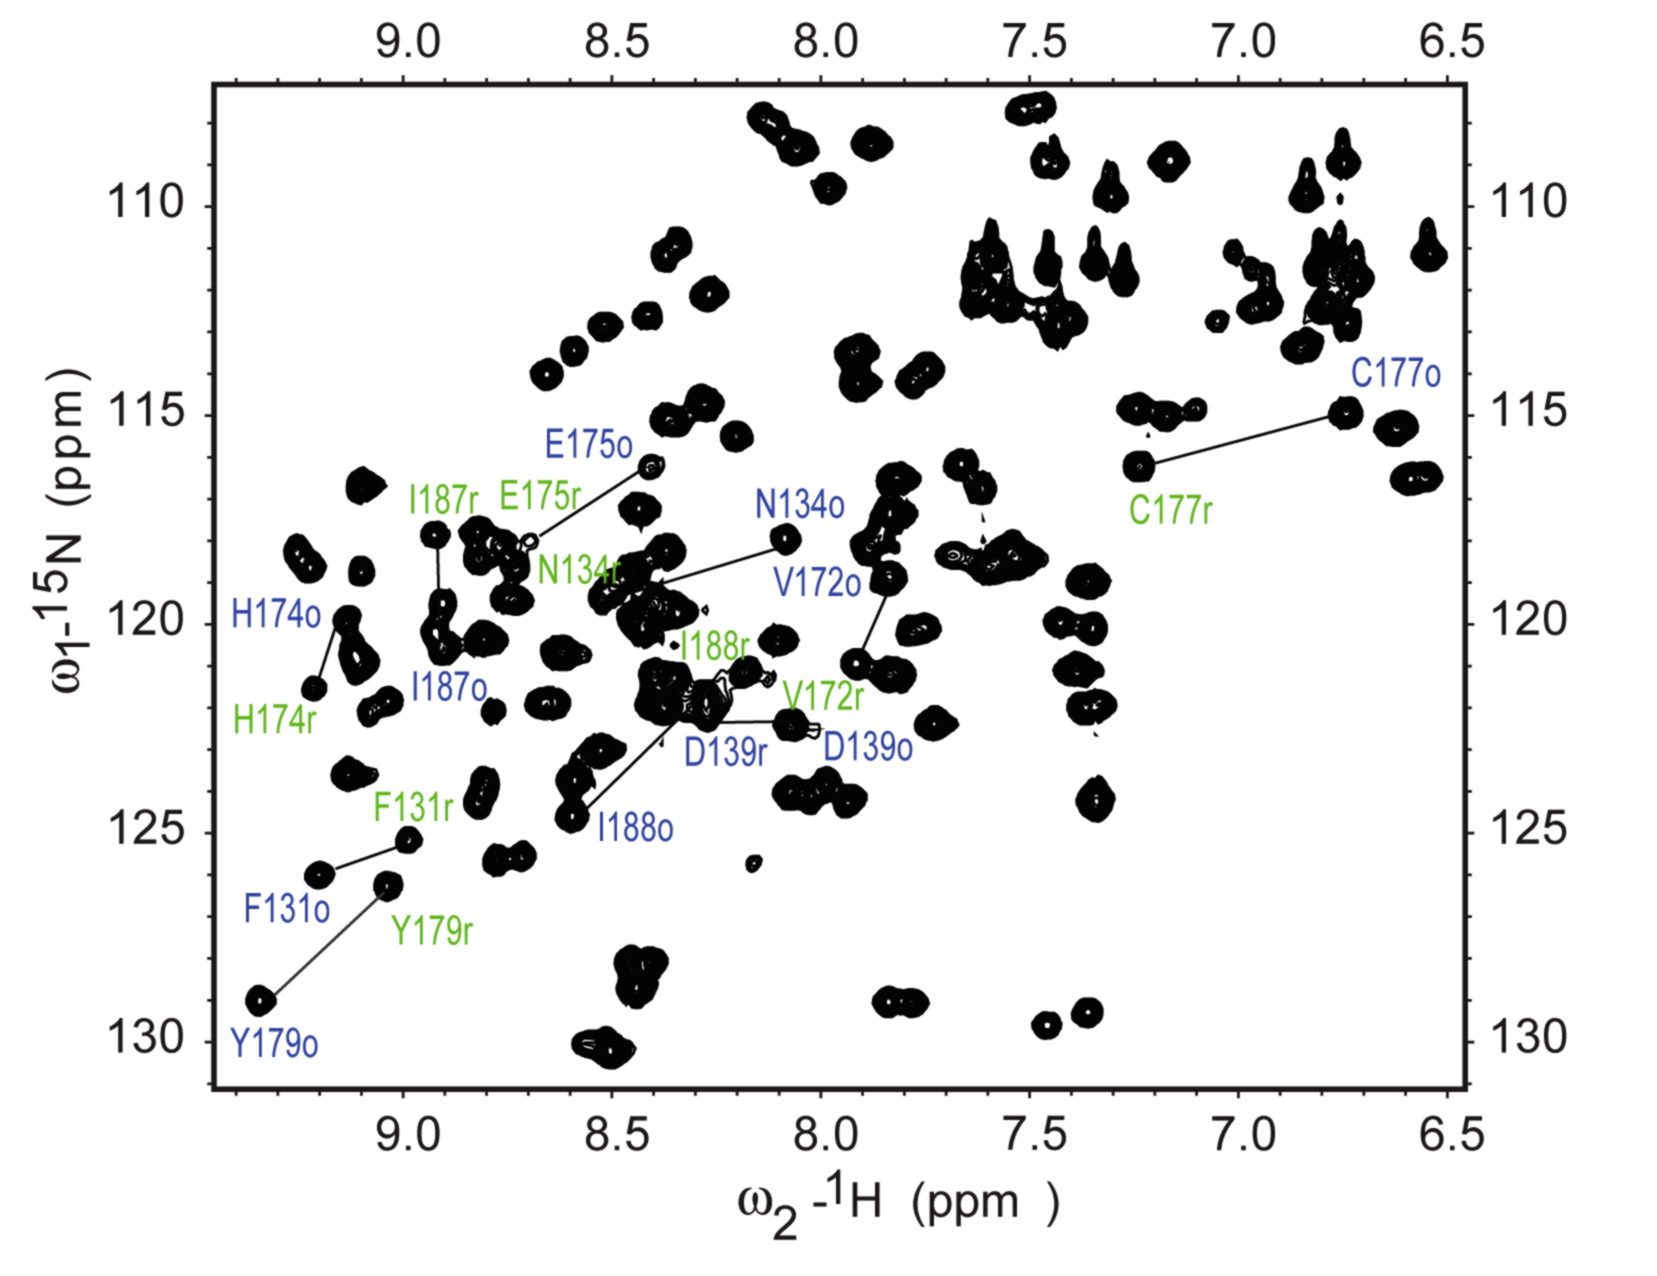
\includegraphics[width=1\textwidth]{NMR.jpg}
    \caption{2D \textsuperscript{15}N-HSQC spectrum of NleG2-3[90–191] at \ang{25}C and pH 7.0. Selected peaks corresponding to reduced and oxidised conformations are labeled as r (green) and o (blue), respectively. The image is reproduced from \url{https://commons.wikimedia.org/wiki/File:HSQC-NMR.tiff} under the Creative Commons Attribution 2.5 Generic license.} 
\label{fig:NMR}
\end{figure}

Solution NMR spectroscopy determines structural information from nuclear spin interactions (\textbf{Figure \ref{fig:NMR}}), like the nuclear Overhauser effects (NOE), scalar couplings, residual dipolar couplings, and chemical shifts. These are translated into distance and angle restraints, from which atomic models are calculated, often yielding an ensemble of conformers consistent with the data\cite{CH4_Ulrich2008_BMRB,CH4_baskaran2024restraint}.  The associated data are archived in the PDB and in the Biological Magnetic Resonance Data Bank (BMRB)\cite{CH4_Ulrich2008_BMRB}, and comprises of the following output:
\begin{itemize}
  \item Structural ensembles deposited as multiple models per PDB entry.
  \item Restraint lists and chemical shifts, which are accessible via BMRB and wwPDB reports.
  \item Validation metrics for both structural geometry and restraint satisfaction.
\end{itemize}

\subsubsection{Validation and Accuracy}
Global analyses of NMR structures reveal that the secondary structure elements are usually well defined, however, the overall structures may be too flexible, particularly in loops and termini, reflecting under-restraint rather than true intrinsic disorder\cite{CH4_fowler2020method,CH4_baskaran2024restraint}. The ensemble RMSD and restraint counts are rough indicators. Whereas the newer methods, such as ANSURR, compare predicted rigidity from the structure to that inferred from chemical shifts, providing more nuanced accuracy estimates\cite{CH4_fowler2020method}. The geometry metrics, such as, the Ramachandran outliers, rotamers, and clashes correlate with better agreement to independent data.\cite{CH4_Williams2018_MolProbity,CH4_baskaran2024restraint}

\subsubsection{Caveats Relevant to Docking}
The NMR structures are particularly valuable for capturing conformational dynamics and alternative states. However, docking workflows must select conformers carefully and, when possible, cross-validate against crystallographic or cryo-EM models. From a docking perspective, NMR structures have characteristics that require special care. Different conformers obtained as ensembles can be equally consistent with experimental restraints, therefore, choosing a single arbitrary conformer may bias docking. The Loops or side chains may be weakly restrained, which are effectively modelled rather than determined. Therefore, these regions may not provide reliable structural informations, moreover, if they occur in the binding site regions, the pocket geometries may not fully correct. Since NMR measurements do not yield density information, there are no electron density or EM maps to inspect. Therefore, the quality must be judged via completeness of the restraints, violations, and comparison to independent data.  While NMR can determine oligomeric complexes, the stoichiometry and symmetry can be underdetermined in some cases.


\subsection{Other Experimental and Integrative Methods}
Several additional biophysical techniques provide structural information that can be important for SBDD:
\begin{itemize}
  \item \textbf{Small-angle X-ray scattering (SAXS) and small-angle neutron scattering (SANS)}: These provide low-resolution shapes and information about global flexibility in solution. The curated SAXS/SANS data and associated models are available in Small Angle Scattering Biological Data Bank(SASBDB)\cite{CH4_Valentini2015_SASBDB,CH4_pesce2021refining}.
  \item \textbf{Hybrid and integrative methods}: Structures may combine X-ray, Cryo-EM, SAXS, cross-linking mass spectrometry, FRET and other data. These are curated in specialised repositories such as PDB-Dev.\cite{CH4_pesce2021refining}
  \item \textbf{Serial and time-resolved crystallography}: These techniques provide snapshots of macromolecular processes at millisecond or faster timescales. However, individual states may be at modest resolution or represent mixtures of conformations.
\end{itemize}

These approaches are rarely used directly as receptor structures for docking. However, they are extremely valuable for validating conformational states sampled in docking or molecular dynamics (MD) that are likely to be relevant in solution.

\section{Structural Data Resources}

\subsection{The wwPDB Ecosystem}

The Worldwide Protein Data Bank (wwPDB) manages the global archives for three-dimensional biomacromolecular structure data.\cite{CH4_Berman2000_PDB,CH4_wwpdb2019protein,CH4_young2018worldwide}. The PDB core archive\cite{CH4_Berman2000_PDB,CH4_wwpdb2019protein} stores atomic coordinates of proteins, nucleic acids, complexes, and their ligands, determined by X-ray, NMR, cryo-EM and other methods. The Electron Microscopy Data Bank(EMDB)\cite{CH4_wwpdb2024emdb} is a repository of three-dimensional cryo-EM reconstructions, is often linked to fitted atomic models. The Biological Magnetic Resonance Data Bank(BMRB)\cite{CH4_Ulrich2008_BMRB} archives NMR chemical shifts, restraints, and related spectroscopic data.
The regional PDB partners (RCSB PDB, PDBe, PDBj, and PDBj-BMRB)\cite{CH4_wwpdb2019protein,CH4_Velankar2016_PDBe} provide portals, visualisation tools, and value-added annotations. The wwPDB provides standardised \emph{validation reports} for X-ray, cryo-EM, and NMR entries, summarising global and local quality metrics.\cite{CH4_karplus2012linking,CH4_shao2017multivariate,CH4_young2018worldwide}


\subsection{PDBe, PDBe-KB, and PISA}
The Protein Data Bank in Europe (PDBe)\cite{CH4_Velankar2016_PDBe} is a major PDB partner that provides high-quality, integrated views of structural data. PDBe and its knowledge base provides an interactive structure viewers and summarised validation metrics. It provides cross-links to functional, sequence, and ligand information. And, integrates access to EMDB, BMRB, SASBDB, and related resources. Of particular importance to docking is PDBePISA (Proteins, Interfaces, Structures and Assemblies)\cite{CH4_Krissinel2007_PISA}, which analyses interfaces, surfaces, and assemblies in crystal structures and predicts likely biological oligomeric states. PDBePISA reports (\textbf{Figure \ref{fig:PISA}}) interface areas, solvation energy gains, hydrogen bonds, salt bridges and hydrophobic contacts, and ranks interfaces according to their probability of being biologically relevant.

\begin{figure}[hbt!]
    \centering
    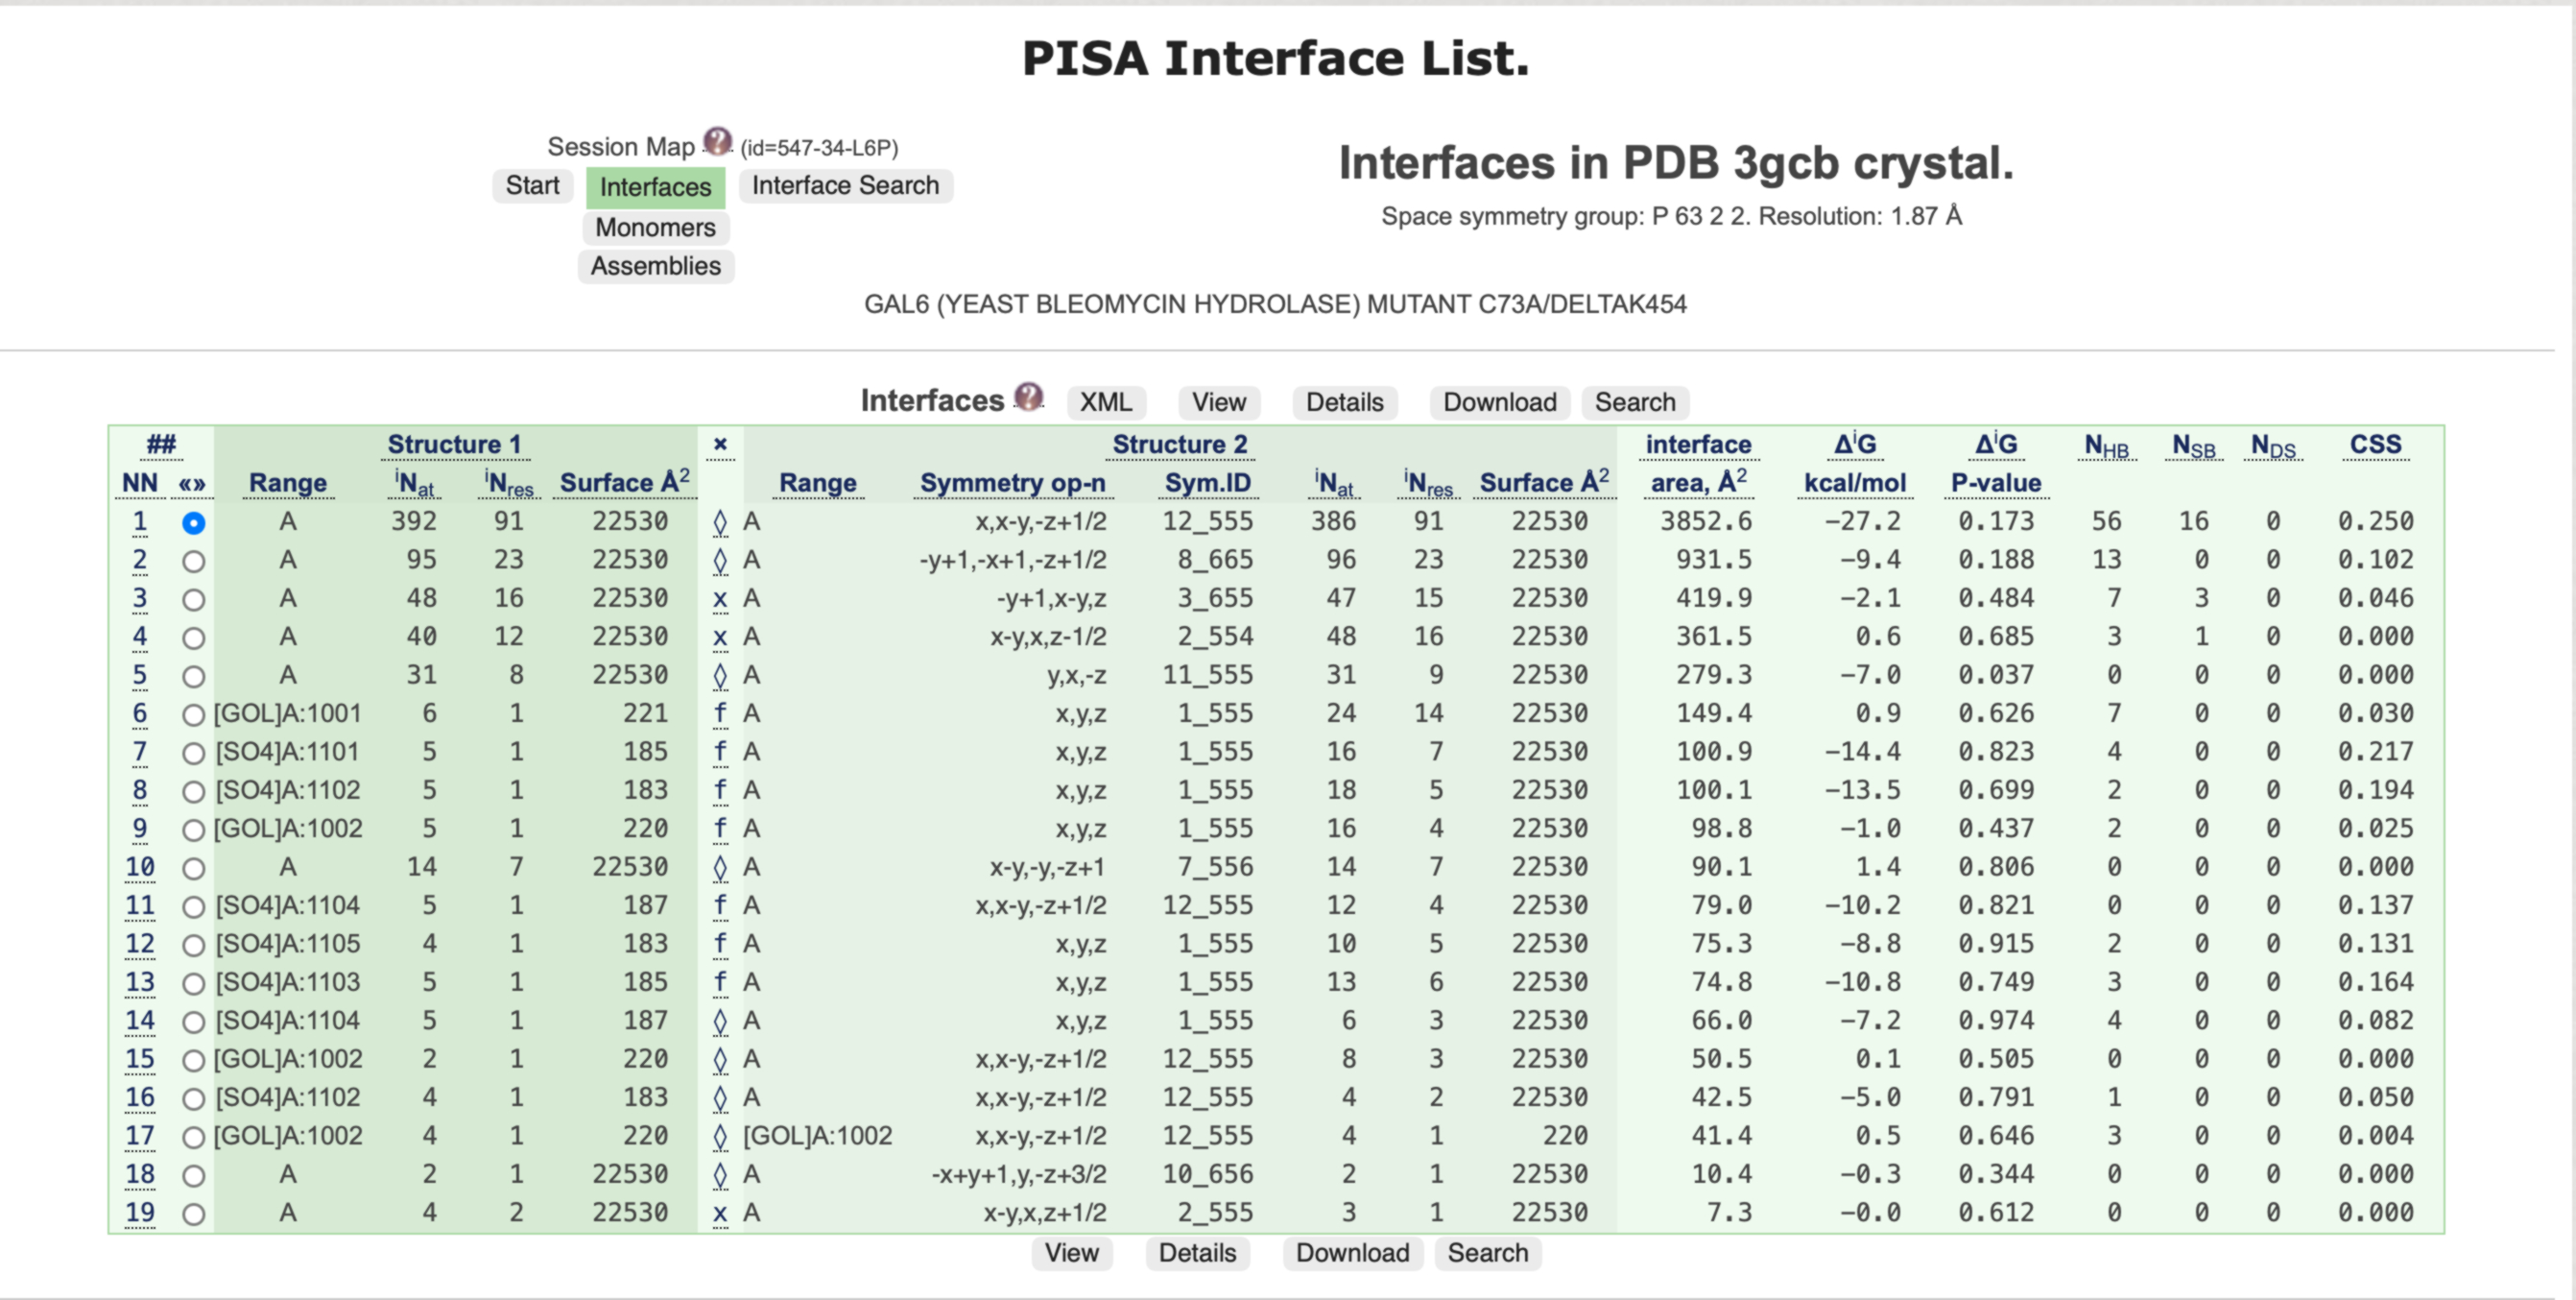
\includegraphics[width=1\textwidth]{PDBPISA.jpg}
    \caption{An example output obtained from the PDBe PISA webserver.}
\label{fig:PISA}
\end{figure}

\subsection{BMRB and associated portals}

BMRB\cite{CH4_Ulrich2008_BMRB} and its Japanese mirror, BMRBj, provide detailed NMR data, including chemical shifts, coupling constants, and restraint lists. These underpin recent wwPDB efforts to validate NMR structures based on restraint violations and consistency between experimental observables and the structural ensemble.\cite{CH4_baskaran2024restraint}
In the context of molecular docking, the structural information can be helpful to assess how well the experimental data constrains an NMR ensemble. It can be provide valuable input to integrating chemical shift-based information on local structure and dynamics with crystallographic or cryo-EM models.

\subsection{EMDB}
The EMDB\cite{CH4_wwpdb2024emdb} provides curated access to three-dimensional EM maps, with associated metadata and validation information. Many PDB entries derived from cryo-EM experiments specify an associated EMDB map identifier, making it straightforward to access the underlying map and validation report. It serves to provide processed maps, and half-maps to assist an independent validation. The global and local resolution estimates are helpful to evaluate the quality of the overall structure, and more importantly, the quality of the binding site. It further serves to provide cross-links to fitted atomic models and related experimental data\cite{CH4_pintilie2021validation}. Therefore, docking users can directly assess whether a particular binding site is supported by strong local density, and whether the fitted ligand or side-chain conformations are justified.

\subsection{Small Angle Scattering Biological Data Bank (SASBDB)}
The SASBDB\cite{CH4_Valentini2015_SASBDB} archives small-angle scattering data and associated structural models. Although docking is rarely performed directly into SAXS-derived models, SASBDB entries can be used to validate whether global conformational states used in docking, compact vs extended, are compatible with solution scattering data. It allows one to assess receptor flexibility, oligomeric states, and the presence of large-scale conformational changes.\cite{CH4_pesce2021refining}

\subsection{PDB-REDO}
PDB-REDO\cite{CH4_Joosten2014_PDBREDO} re-refines, and partially rebuilds macromolecular crystallographic structures using updated refinement protocols and model-building tools. Its key features include:

\begin{itemize}
  \item Systematic optimisation of refinement parameters, anisotropic scaling, and B-factor models.
  \item Automated correction of side-chain conformations, peptide flips, and local geometry problems.
  \item Improved R-factors and stereochemical quality in many cases, often without worsening fit to experimental data.
\end{itemize}

For docking and SBDD, PDB-REDO models often provide superior starting points than the original PDB entries, especially for older structures refined with now-outdated methods.

\subsection{AlphaFold protein structure database}

\begin{figure}[hbt!]
    \centering
    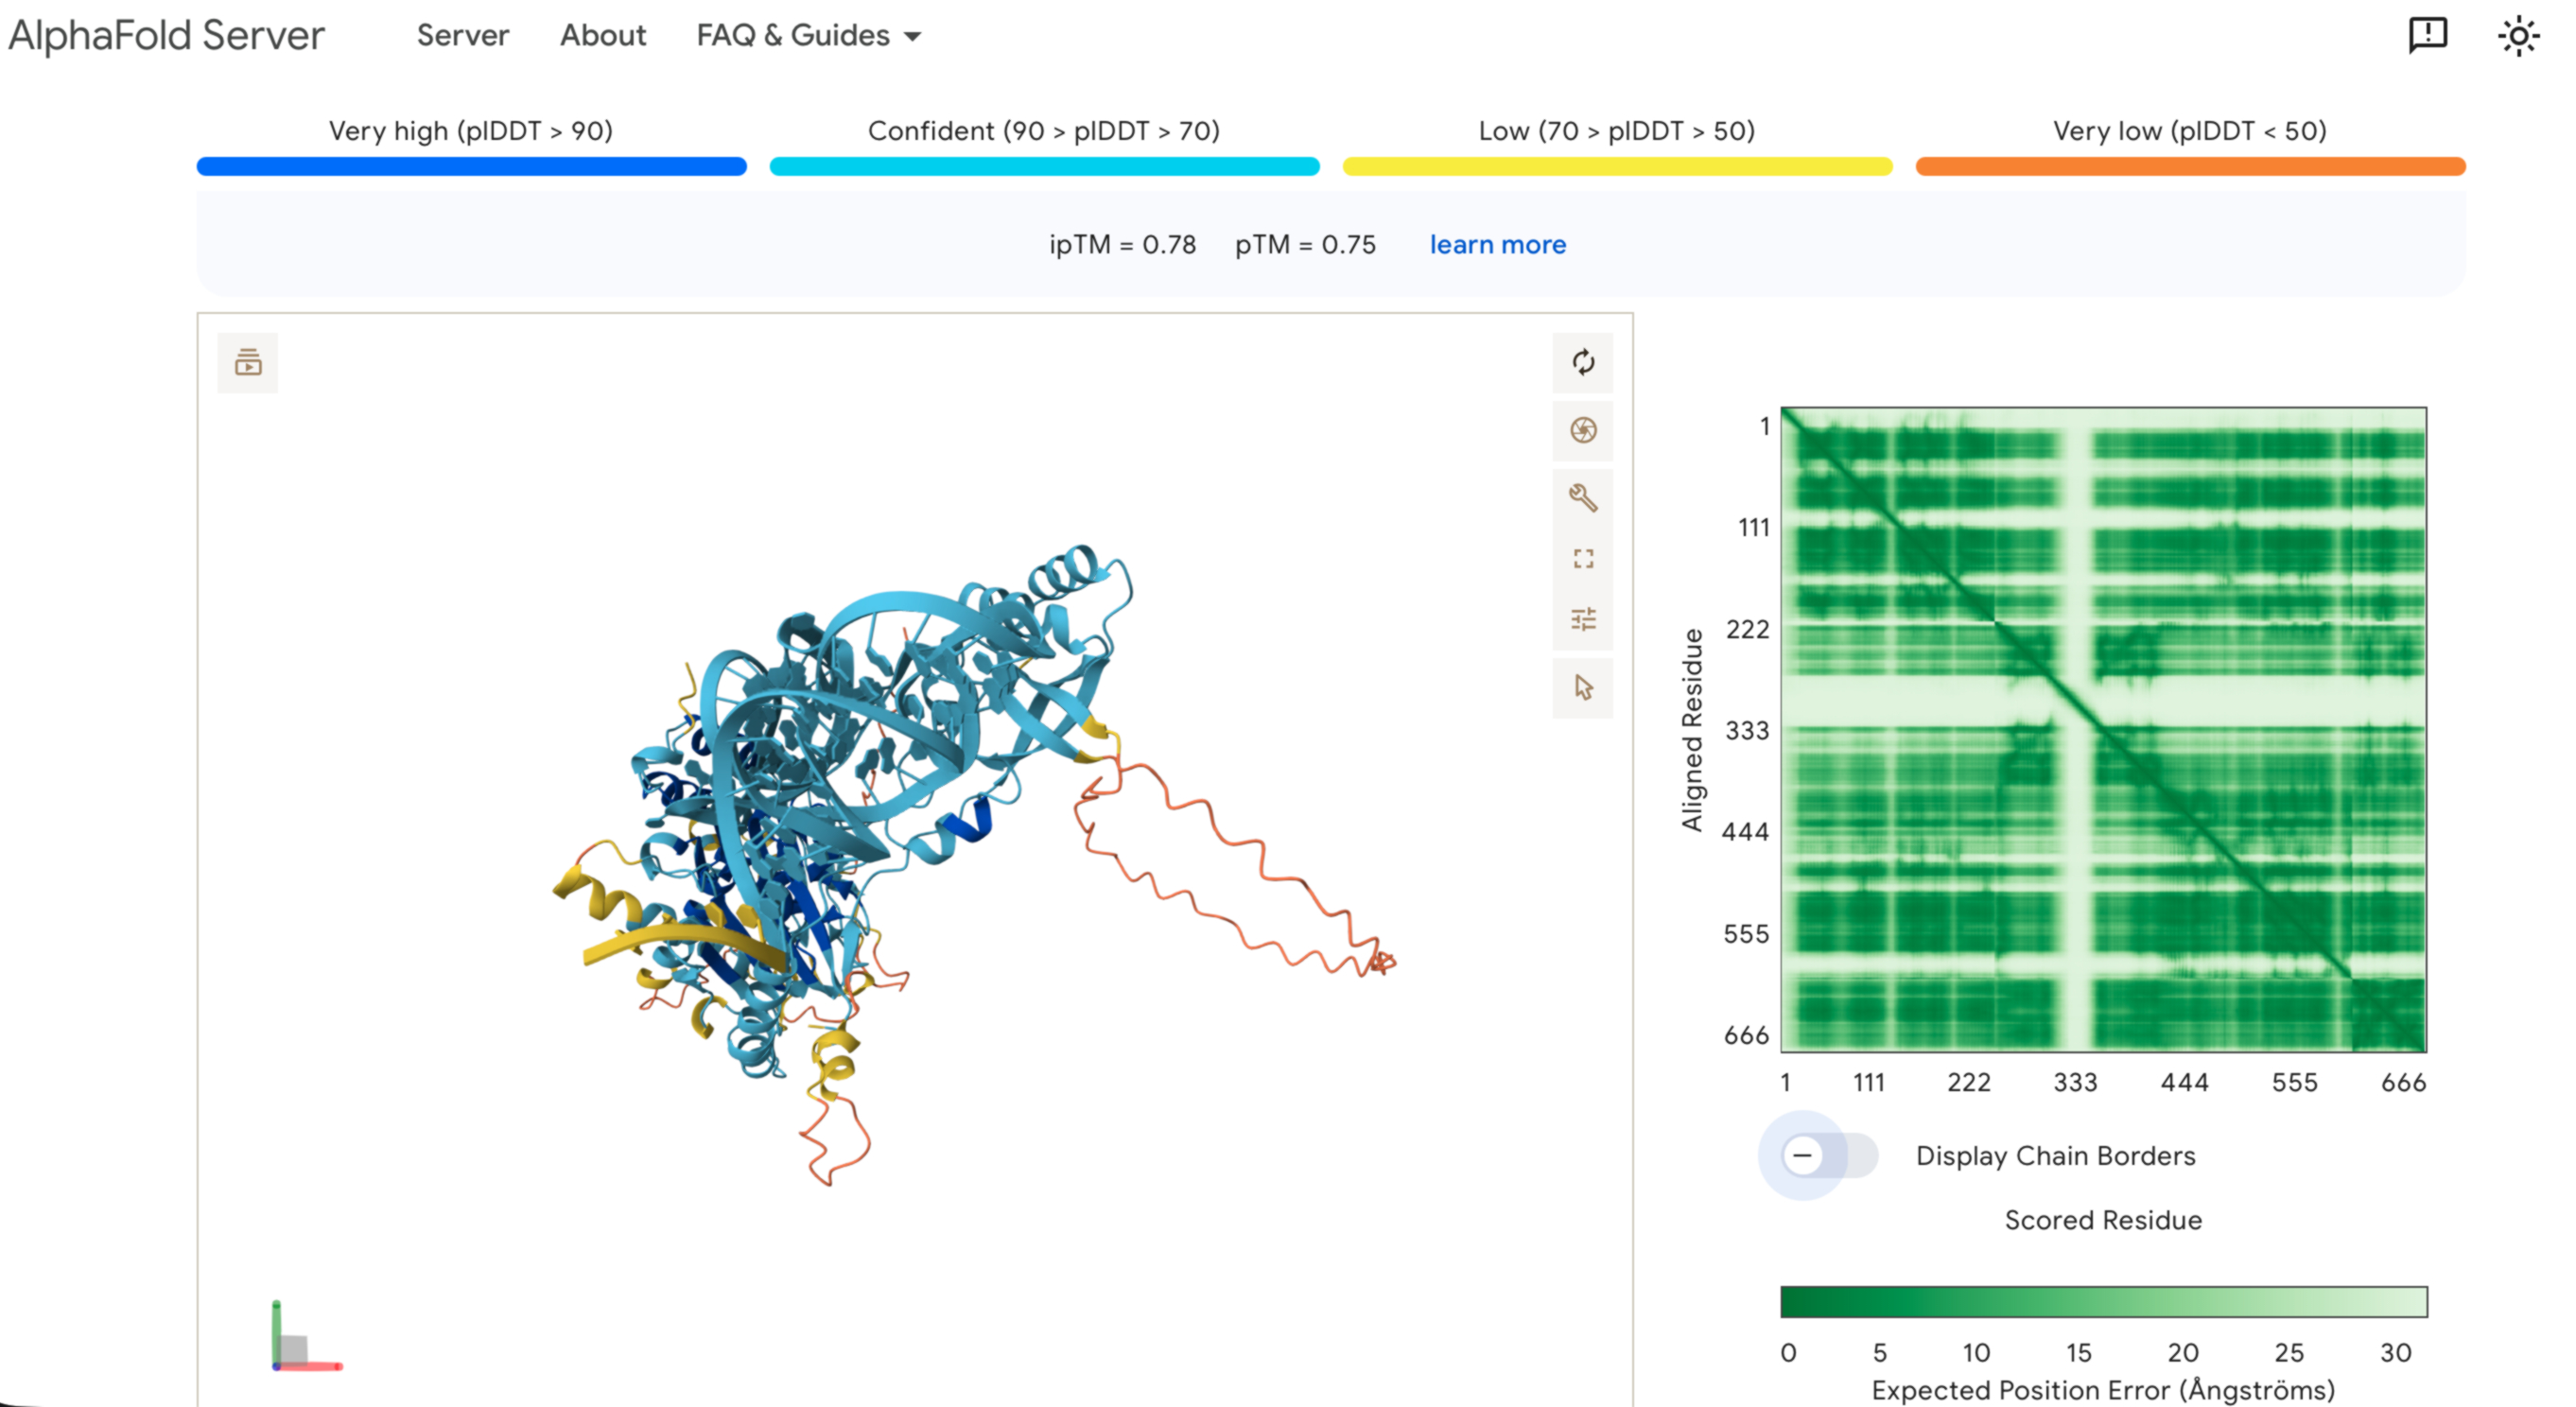
\includegraphics[width=1\textwidth]{AF3.jpg}
    \caption{An example output for protein-DNA complex prediction from the Alphafold3 server.}
\label{fig:AF3}
\end{figure}

The AlphaFold\cite{CH4_Jumper2021_AlphaFold,CH4_Varadi2022_AlphaFoldDB} Protein Structure Database provides \emph{in silico} structural models for a large fraction of many reference proteomes, generated using AlphaFold2 (\textbf{Figure \ref{fig:AF3}}). These models are accompanied by per-residue confidence scores (pLDDT) and predicted aligned error (PAE) matrices. From a docking perspective, AlphaFold models have several important features\cite{CH4_Jumper2021_AlphaFold,CH4_Varadi2022_AlphaFoldDB}.  For many globular domains, regions with high pLDDT (typically $>$70--80) tend to have near-experimental backbone accuracy. The PAE provides information about uncertainty in relative domain orientations. A high PAE indicates that domain arrangements may be incorrect even if individual domains are accurate. Ligands, cofactors, metals, and PTMs are \emph{not} modelled; pockets that depend on these features may have incorrect shapes or be absent. The multimer predictions (AlphaFold-Multimer) are less reliable than monomeric predictions, particularly for weak or transient interfaces. The predicted structures should. therefore, be used with caution in docking. They are particularly valuable when no experimental structures are available, however, one must filter by confidence metrics and, where possible, cross validate against functional and other structural data.\cite{CH4_Varadi2022_AlphaFoldDB}


\section{Working with Structural Data}
This section presents a step-by-step workflow for preparing biomacromolecular structures for docking and SBDD. The steps focus on issues most likely to affect binding-site shape, polarity, and dynamics, and thus the accuracy of the docking outcomes.

\subsection{Verify Structure Resolution and Quality Metrics}

\subsubsection{X-ray Structures}
When evaluating an X-ray structure as a receptor, the following checks are recommended:

\begin{itemize}
 \item \textbf{Global resolution and R-factors}: Using the PDB or PDBe entry, note:

\begin{itemize}
  \item The reported resolution limit (highest resolution shell).
  \item $R_\text{work}$ and $R_\text{free}$, and their difference $\Delta R = R_\text{free} - R_\text{work}$.\cite{CH4_Wang2015_structure_quality,CH4_karplus2012linking}
  \item Data completeness and $\textrm{CC}_{1/2}$ in the highest resolution shell\cite{CH4_Evans2013_data_quality,CH4_Read2011_CC12}.
\end{itemize}

A structure with resolution better than about 2.5 \r{A}, complete data, and reasonable R-factors is generally suitable as a starting point, though local issues may still be present\cite{CH4_Wang2015_structure_quality,CH4_shao2017multivariate}. Extremely large $\Delta R$ values ($>$0.07) or very poor R-factors for the nominal resolution suggest either problematic data or overfitted/underfitted models.

% put figure for validation slider
 \item \textbf{Validation \emph{slider} summaries}: wwPDB validation reports present percentile-based sliders for global metrics such as geometry, clashes, R-factors, and more, relative to all structures and to structures at similar resolution.\cite{CH4_karplus2012linking,CH4_shao2017multivariate,CH4_young2018worldwide} Prefer entries where:

\begin{itemize}
  \item Geometry and clashscore are within good percentiles.
  \item R-factors are not severe outliers for the given resolution.
\end{itemize}

 \item \textbf{Local quality near the binding site}: Global metrics can hide serious local problems\cite{CH4_chakraborti2021all,CH4_shao2017multivariate}. Most PDB and PDBe viewers allow the user to:
\begin{itemize}
  \item Map per-residue real-space correlation coefficients or B-factors onto the structure.
  \item Identify outliers (clashes, Ramachandran and rotamer outliers) near the binding site.
\end{itemize}

\subsubsection{Cryo-EM Structures}
For structures derived from cryo-EM:
 \item \textbf{Global and local resolution}: The following checks must be performed:

\begin{itemize}
  \item The global FSC-based resolution and the FSC curve, noting the threshold used.
  \item Local resolution maps to determine whether the binding-site region has comparable or worse resolution than the global value.
\end{itemize}

 \item \textbf{Map--model validation}: Evaluate:
 
\begin{itemize}
  \item Real-space correlation coefficients per residue and per ligand.
  \item Local map-to-model quality metrics such as Q-scores.\cite{CH4_Pintilie2020_Qscore,CH4_pintilie2021validation}
  \item Geometry metrics (Ramachandran, rotamers, clashes) in the binding-site region.\cite{CH4_Williams2018_MolProbity}
\end{itemize}
\end{itemize}

If the pocket is situated in a low-resolution region or shows poor map support for key residues and ligands, the structure may be unsuitable for docking, and yield unreliable results. 

\subsubsection{NMR Structures}

For NMR-derived structures:

\begin{itemize}
  \item \textbf{Ensemble and restraint statistics}: Examine:

\begin{itemize}

  \item The ensemble RMSD, particularly for backbone atoms in the folded structure.
  \item The number and type of restraints (NOEs, RDCs) per residue.
  \item Restraint violation statistics from wwPDB or BMRB reports.\cite{CH4_baskaran2024restraint}

\end{itemize}

  \item \textbf{Geometry and accuracy assessments}: Use wwPDB validation reports and specialised tools such as ANSURR:\cite{CH4_fowler2020method,CH4_Williams2018_MolProbity}

\begin{itemize}
  \item Ensure Ramachandran and rotamer outliers are minimal in the binding-site region.
  \item Verify that the rigidity inferred from chemical shifts (ANSURR) is consistent with the modelled structure in key regions.\cite{CH4_fowler2020method}
\end{itemize}
\end{itemize}

For docking, it is often prudent to select a subset of conformers that best represent compact, well-defined pocket geometries, guided by restraints and functional data.

\subsection{Identify and Fix Missing Residues}
Most macromolecular structures have missing residues: segments present in the SEQRES sequence but absent from the ATOM records. These may be flexible loops, termini, or regions disordered under the experimental conditions.

\begin{itemize}
\item \textbf{Identify missing segments}: PDB and PDBe pages list missing residues explicitly. Consider:

\begin{itemize}
  \item N- and C-terminal regions, which often have limited functional impact.
  \item Internal loops proximal to the binding site, which can gate access or contribute directly to ligand recognition.
  \item Missing side chains from incomplete modelling of long side chains, such as lysine or arginine. These are generally observed when the residues with long side chains are solvent exposed and highly dynamic.

\end{itemize}

\item \textbf{Assess functional impact}: Determine whether the missing region:

\begin{itemize}
  \item Lines the binding pocket.
  \item Controls access to the site (e.g. an activation loop).
  \item Participates in oligomeric contacts that shape the binding site.
\end{itemize}

\item \textbf{How to handle missing regions?}:

\begin{itemize}
  \item Ignore remote, non-critical segments: Terminal regions far from the binding site can often be neglected, unless one wishes to perfomed MD simulations after docking.
  \item To model critical loops and segments, use homology modelling or loop-building tools, ideally guided by related high-resolution structures. Or use AlphaFold or AlphaFold-Multimer predictions\cite{CH4_Jumper2021_AlphaFold,CH4_Varadi2022_AlphaFoldDB}, carefully aligned and grafted onto the experimental model, guided by pLDDT and PAE to gauge confidence.
  \item Constrain docking away from uncertain regions If reliable modelling is not possible, restrict docking to regions whose shapes are experimentally supported.
\end{itemize}
\end{itemize}

\subsection{Differentiating Crystal Packing Multimers from Biological Multimers}
The asymmetric unit of a crystal is not necessarily the biological oligomeric state. For docking, especially at protein--protein interfaces or quaternary allosteric sites, using the correct biological assembly is essential.

\begin{itemize}
\item \textbf{Asymmetric unit vs biological assembly}: PDB entries specify the \emph{asymmetric unit} (ASU), the minimal crystallographic repeating unit. Futhermore, the transformation matrices (BIOMT/BIOMATRIX) defines the putative biological assemblies.

\item \textbf{Use PDBePISA to analyse interfaces}: The PDBePISA\cite{CH4_Krissinel2007_PISA} evaluates crystal packing interfaces and predicts likely biological oligomers. It reports the buried surface area and solvation free-energy gain ($\Delta \textrm{G}$) upon complex formation. It shows the hydrogen bonds, salt bridges, and hydrophobic contacts. It also provides a probability score for each interface being biologically significant. Interfaces with large buried surface area, favourable $\Delta \textrm{G}$, and hydrophobic cores are more likely to be physiological relevant. Whereas small, polar contacts are more likely to be crystal artefacts.

\item \textbf{Use independent interface discrimination methods}: Methods that examine shape complementarity, conservation, and physicochemical complementarity can distinguish biological from crystal contacts.

\item \textbf{Cross-check with solution data}: When possible, compare with:
\begin{itemize}
  \item Size-exclusion chromatography, analytical ultracentrifugation.
  \item SAXS\cite{CH4_Valentini2015_SASBDB,CH4_pesce2021refining} profiles and envelopes.
  \item NMR data\cite{CH4_Ulrich2008_BMRB}, such as, the chemical shift perturbations upon oligomerisation.
\end{itemize}

For docking at interfaces, it always recommended to construct the predicted biological assembly, rather than using the ASU by default.

\subsection{Understanding B-factors and Crystal Packing Effects on Dynamics}
B-factors (atomic displacement parameters) quantify the mean-square displacement of atoms from their average positions in the model. They reflect a combination of physical motion, static disorder, and model uncertainty.

\item \textbf{Interpretation within a single structure}: Within one structure,  the relative B-factors can help identify rigid cores (low B-factors) and flexible loops or termini (high B-factors). However, very high B-factors or partial occupancy on ligands and side chains suggest poorly defined positions. The B-factors are influenced by refinement choices, such as individual vs group refinement, TLS models, resolution, and should not be interpreted as quantitative measures of physical mobility.\cite{CH4_Wang2015_structure_quality,CH4_shao2017multivariate}

\item \textbf{Crystal packing effects}: The lattice contacts can stabilise conformations that are less populated in solution.  These will often have relatively low B-factors despite being constrained by non-physiological interactions. Conversely, some high B-factors reflect poor data quality at the resolution limit rather than true dynamics.\cite{CH4_Evans2013_data_quality,CH4_Joosten2009_PDB_related_databanks} Cryo-EM models often use sharpened B-factors that reflect map processing rather than atomic mobility, and thus need to be interpreted cautiously.\cite{CH4_pintilie2021validation}


\item \textbf{Implications for docking}: Use B-factors as a qualitative guide:

\begin{itemize}
  \item High B-factors on side chains directly involved in ligand binding indicate uncertainty in their orientations. These may need to be sampled during docking or MD simulations.
  \item Low B-factors in the core support more rigid-body treatments, at least within a given conformational state.
\end{itemize}
\end{itemize}

Combine B-factors with ensemble information from multiple structures, NMR, and MD simulations to decide which regions should be treated as flexible in docking protocols.

\subsection{Model Non-Standard Residues }

Many drug targets carry Post-Translational Modifications (PTMs) or bind essential cofactors, metals, lipids, or glycans. Experimental structures may incompletely capture the PTMs which should be explicitly modelled using modified residue codes (e.g. SEP for phosphoserine). Glycan chains may be truncated when appropriate. The essential cofactors or metals might be absent in apo structures or replaced by analogues which must added to the correct site. Certain mutations may be inserted to aid crystallisation may alter local structure, these mutations should reverted to wild-type amino acid.

\begin{itemize}
  \item \textbf{Identify non-standard residues and cofactors}: Examine \emph{HETATM} records and ligand lists in PDB/PDBe entries:
\begin{itemize}
  \item Distinguish biologically relevant components (ATP, NAD\textsuperscript{+}, Zn\textsuperscript{2+}, heme, lipids) from crystallisation artefacts (sulfate, glycerol, polyethene glycol).
  \item Use LINK records and annotations to identify PTMs and covalent linkages.
\end{itemize}

  \item \textbf{Model missing PTMs and cofactors}: If biochemical data indicate that a PTM or cofactor is essential for function but absent from the structure, one may consider to graft the PTM or cofactor from a related structure, such as a homologue or another conformational state. Positioning it may be based on conserved sequence motifs, coordination geometry, and electrostatics. And lastly, validate the geometry against small-molecule crystallographic distributions using tools such as Mogul\cite{CH4_bruno2004retrieval,CH4_nicholls2017ligand}.

  \item \textbf{Parameterisation for docking}: Non-standard residues, PTMs, and cofactors often require parameter generation for docking and MD:
\begin{itemize}
  \item Use small-molecule parameter generators (e.g. AceDRG\cite{CH4_long2017}, automated-topology builder (ATB)\cite{CH4_stroet2018}, antechamber\cite{CH4_wang2001}) or quantum chemistry-derived parameters consistent with the force field.\cite{CH4_nicholls2017ligand,CH4_bruno2004retrieval}
  \item Ensure charges and protonation states are appropriate for the physiological pH and binding environment.
\end{itemize}
\end{itemize}
As a rule, keep biologically essential PTMs and cofactors in the model, and exclude obvious crystallisation artefacts unless one needs to explicitly model their effects.

\subsection{Validate Ligand and Cofactor Binding Sites and Geometries}
Ligand models in PDB structures range from excellent to seriously flawed. Incorrect ligand geometries or poses will mislead docking and SBDD.\cite{CH4_chakraborti2021all,CH4_emsley2017tools}

\begin{itemize}
\item \textbf{Density support}: For X-ray structures:
\begin{itemize}
  \item Inspect 2$\textrm{F}_\textrm{o}-\textrm{F}_\textrm{c}$ and $\textrm{F}_\textrm{o}-\textrm{F}_\textrm{c}$ maps around the ligand using Coot\cite{CH4_Emsley2010_Coot} or other viewers.
  \item Check for continuous, well-defined 2$\textrm{F}_\textrm{o}-\textrm{F}_\textrm{c}$density surrounding the ligand, and absence of strong negative $\textrm{F}_\textrm{o}-\textrm{F}_\textrm{c}$ peaks on ligand atoms.
  \item Use residue-level density metrics, such as real-space correlation, and real-space R-factors, when available.\cite{CH4_karplus2012linking,CH4_Joosten2014_PDBREDO}
\end{itemize}

For cryo-EM structures, examine the EMDB map in the binding-site region and ensure the ligand is supported by clear density, rather than being floated into weak or noisy features.\cite{CH4_pintilie2021validation}

\item \textbf{Geometry and conformation}: Assess ligand geometry using:
\begin{itemize}
  \item Internal bond lengths, angles, and ring conformations.
  \item Comparison to distributions from small-molecule databases (e.g. Mogul)\cite{CH4_bruno2004retrieval}.
  \item Tools like Coot and CCP4 for ligand validation and refinement\cite{CH4_emsley2017tools,CH4_nicholls2017ligand}.
\end{itemize}
Distorted geometries or unnatural ring conformations not justified by strong interactions suggest mis-modelling.

\item \textbf{Interactions and environment}: Evaluate:
\begin{itemize}
  \item Hydrogen-bonding patterns, salt bridges, and hydrophobic contacts.
  \item Consistency with known structure--activity relationships (SAR) and mutagenesis data.
  \item Ligand B-factors and occupancy relative to surrounding residues.
\end{itemize}

Ligands with very high B-factors or low occupancy may represent partial binding or multiple orientations.

\item \textbf{Receptor selection for docking}: Prefer complexes where:
\begin{itemize}
  \item Ligand density is strong and unambiguous.
  \item Ligand geometry is plausible and supported by small molecule statistics.
  \item Binding interactions align with SAR and functional data.
\end{itemize}
\end{itemize}



\subsection{Check Experimental Methods and Their Limitations}
The suitability of a structure for docking depends on its determination method:

\begin{itemize}
  \item \textbf{X-ray crystallography}: It provides high spatial resolution but is subject to crystal packing, cryogenic artefacts, and model bias; ligands can be over-interpreted if density is weak.\cite{CH4_Evans2013_data_quality,CH4_karplus2012linking,CH4_chakraborti2021all}

  \item \textbf{Cryo-EM}: It is powerful for large complexes and membrane proteins, but map quality is locally variable; flexibility can obscure side chains and ligands.\cite{CH4_pintilie2021validation}

  \item \textbf{NMR}: It captures solution dynamics and ensembles, but some regions may be under-defined. The global folds of large complexes can be challenging to determine.\cite{CH4_Ulrich2008_BMRB,CH4_fowler2020method}

  \item \textbf{Predicted structures} (e.g. AlphaFold)\cite{CH4_Jumper2021_AlphaFold,CH4_Varadi2022_AlphaFoldDB}: It can be very accurate for many monomeric domains, but uncertain for disordered regions, multi-domain arrangements, complexes, and ligand-dependent pockets.
\end{itemize}

Selection of the receptor structure should take following limitations into account:
\begin{itemize}
  \item For an enzyme with multiple high-resolution X-ray complexes, choose the structure that best reflects the ligand chemotype and functional state of interest.
  \item For a membrane receptor available only in cryo-EM form, examine local map quality, and use AlphaFold predictions and NMR/SAXS data to refine loops and termini.
  \item For intrinsically disordered proteins, neither crystallography nor AlphaFold will provide a stable pocket; docking may be uninformative without additional constraints.
\end{itemize}


\section{Working with Computed Structure Models from the Protein Data Bank}
For decades, structural biology has relied primarily on experimentally determined macromolecular structures deposited in the Protein Data Bank (PDB), including X-ray crystallography, nuclear magnetic resonance (NMR) spectroscopy, and, more recently, cryo-electron microscopy (cryo-EM).\cite{CH4_Berman2000_PDB,CH4_wwpdb2019protein} These experimental structures have enabled structure-based drug design, functional annotation, and mechanistic understanding across essentially all areas of biology. However, experimental structure determination remains costly and time-consuming, and many proteins — especially membrane proteins, large complexes, and intrinsically disordered regions — remain structurally uncharacterised.

Recent advances in machine-learning-based structure prediction, most prominently AlphaFold2\cite{CH4_Jumper2021_AlphaFold,CH4_Varadi2022_AlphaFoldDB} and related methods, have transformed this landscape. High-accuracy \emph{computed structure models} (CSMs) can now be generated at scale, and millions of predicted protein structures are accessible through resources that are integrated with, or closely linked to, the PDB. RCSB PDB, PDBe, and wwPDB partners now provide portals where users can browse both experimentally determined structures and CSMs side by side.\cite{CH4_wwpdb2019protein,CH4_Burley2022}


\subsection{Accessing Computed Structure Models}

The wwPDB partners collaborate with external CSM providers, such as the AlphaFold DB and RoseTTAFold servers, to make predicted structures discoverable through familiar PDB interfaces.\cite{CH4_wwpdb2019protein,CH4_Varadi2022_AlphaFoldDB} A typical access pattern is:
\begin{itemize}
  \item A user searches for a protein of interest using a PDB portal (e.g. RCSB PDB or PDBe), by name or by UniProt accession.
  \item If experimental structures are available, they are listed first, often with associated ligands, complexes, and validation metrics.
  \item In addition, a \emph{Computed Structure Models} section highlights links to AlphaFold or other prediction resources, with direct download options for the predicted structures.

\end{itemize}

This approach has several advantages, such as, it keeps the PDB archive itself focused on experimental entries, preserving historical continuity and validation frameworks. However, it allows users to easily discover CSMs when no experimental structure exists, or when only fragmentary experimental coverage is available. This facilitates comparisons between experimental and computed models, for example, overlaying an AlphaFold model with a partial crystal structure to assess how well predicted domains align with experimental density. The PDB and its partners databases clearly label CSMs as predicted, and typically direct users to the originating resource (e.g. AlphaFold DB) for detailed information on prediction methods, confidence metrics, and licensing.\cite{CH4_Varadi2022_AlphaFoldDB,CH4_Burley2022}

\subsection{Interpreting Confidence Metrics in Computed Models}

The main challenge in working with CSMs is that there are no experimental structure factors or EM maps to validate against. Instead, users must rely on internal confidence measures and external comparisons to experimental structures and functional data.
\subsubsection{Per-residue Confidence: pLDDT}

AlphaFold2\cite{CH4_Jumper2021_AlphaFold,CH4_Varadi2022_AlphaFoldDB} introduces the per-residue predicted local-distance difference test (pLDDT) score, which estimates the expected accuracy of local structure. In practice, the pLDDT values $>$70--80 typically indicate high confidence in the backbone conformation for globular regions. Whereas, lower pLDDT values suggest uncertainty. However, it has been noted that such residues may be disordered, or the model may not have converged on a unique conformation. Many PDB-linked viewers colour code the structure according to pLDDT, making it straightforward to identify well-defined cores vs flexible or poorly predicted regions.

For docking and functional interpretation, pLDDT is a useful first filter. The residues in high-confidence regions can generally be treated as structurally reliable, whereas low-confidence segments should be treated cautiously, modelled flexibly, or excluded from detailed interpretation if far outside the region of interest (binding site).

\subsection{Domain-level Confidence: Predicted Aligned Error (PAE)}

AlphaFold's\cite{CH4_Jumper2021_AlphaFold} predicted aligned error (PAE) matrix encodes anticipated positional errors between residue pairs under an optimal superposition. This provides information about relative domain orientations, such that, low PAE between two domains suggests that their relative placement is predicted with confidence. Whereas, high PAE indicates that the model is uncertain about how domains pack relative to each other, even if each domain individually has high pLDDT. Through PDB-linked viewers or AlphaFold DB itself, users can visualise the PAE matrix interactively. For example, a particular enzyme domain \emph{A}, and another domain \emph{B} may each be well predicted, however, the PAE matrix might reveal that their relative orientation is uncertain. For docking, this implies caution when interpreting inter-domain interfaces or using them as rigid scaffolds.

\subsection{Using Computed Models}

\subsubsection{Model Selection}

When multiple CSMs are available, model selection is guided by the coverage of the region of interest (e.g. inclusion of a particular domain or motif). High pLDDT values in the binding site or functional interface should be preferred. And, low PAE between interacting domains that form the pocket are highly recommended.  Often, the first practical step is to \emph{trim} the model by removing the low-confidence N- and C-terminal regions that are likely to bedisordered and irrelevant for the analysis. Furthermore, consider deleting linkers or insertions with very low pLDDT that do not contribute directly to binding. Such trimming simplifies tasks such as docking and molecular dynamics (MD), while focusing computational efforts on the high-confidence low-error regions of the model.

\subsubsection{Aligning Computed and Experimental Structures}

Computed models can complement experimental structures in the following ways:
\begin{itemize}
  \item Filling gaps where experimental structures lack certain domains or loops.
  \item Suggesting alternative conformational states not captured in crystals or cryo-EM reconstructions.
  \item Providing starting models for experimental phasing or for integrative modelling.
\end{itemize}
Overlaying an AlphaFold model with an experimental structure in the PDB portals allows users to assess how well predicted and observed regions agree\cite{CH4_Varadi2022_AlphaFoldDB,CH4_Burley2022}. Systematic deviations might reveal crystallisation artefacts, domain rearrangements, or functional state differences. Conversely, good agreement increases confidence in using the computed model to extend or interpret the experimental data.

\subsubsection{Incorporating Ligands, Cofactors, and PTMs}

By default, most CSMs do not contain ligands, metal ions, cofactors, or post-translational modifications (PTMs).  When working through PDB-related interfaces, users must therefore,  identify biologically essential ligands and cofactors from experimental structures, UniProt annotations, or biochemical data. It is feasible and advised to manually \emph{graft} these components onto the computed model by aligning to related PDB entries or by docking them into the predicted pocket. Manually modify the natural amino acids to insert PTMs, and parameterise them appropriately for MD or docking.

\subsubsection{Docking and MD with Computed Models}
Computed models can be used as receptors for docking and as starting points for MD simulations. However, we recommend exercising caution at every step to ensure the correction and biological validity of the model(s). Docking into a purely computed pocket is most reliable when pLDDT is high, and the pocket is defined by conserved structural motifs (e.g. catalytic triads, metal-binding sites). For flexible loops or uncertain domains, ensemble docking or enhanced-sampling MD simulations can be used to explore alternative conformations. Moreover, we recommend short MD simulations to relax strained local geometries in computed models and reveal whether the predicted pocket is stable. Since CSMs are not constrained by experimental density, it is particularly important to validate docking results against orthogonal data, such as mutagenesis, SAR, or biochemical assays, before drawing conclusions.

\subsection{Limitations and Best Practices}
While the high accuracy of many CSMs is impressive, they also have systematic limitations:

\begin{itemize}
  \item \textbf{No direct experimental validation:} Confidence metrics such as pLDDT and PAE are internal to the prediction model, and hence, they do not replace experimental verification.
  \item \textbf{Uncertain complexes and interfaces:} Multimer predictions can be less reliable than monomeric models, and many PDB portals distinguish clearly between experimental complexes and predicted oligomeric assemblies.
  \item \textbf{Absence of ligands and PTMs:} As noted, most CSMs lack explicit ligands and modifications, which must be introduced and validated separately.
  \item \textbf{Disordered regions:} Low-pLDDT regions often correspond to intrinsically disordered segments, where a single static model is not a meaningful representation of biological state.
\end{itemize}

Best practices for working with CSMs from PDB-related portals, therefore, include:

\begin{itemize}
  \item Always check and interpret confidence metrics before using a CSM.
  \item Prefer experimental structures where available for the same region and functional state.
  \item Use computed models to fill structural gaps, generate hypotheses, and guide experiments, rather than as a final arbiter of structural truth.
  \item Validate important conclusions against experimental data wherever possible.
\end{itemize}

\section{Summary}

Biomacromolecular structures from X-ray crystallography, cryo-EM, NMR, and prediction methods such as AlphaFold are indispensable for modern SBDD workflows. The quality, completeness, and interpretation of these models, especially in the binding-site region, have profound effects on the docking outcomes. The wwPDB ecosystem and derived databanks now provide rich validation tools, updated models (PDB-REDO), integrative views (PDBe, PDBe-KB), and complementary experimental data (EMDB, BMRB, SASBDB).\cite{CH4_wwpdb2019protein,CH4_Velankar2016_PDBe,CH4_young2018worldwide,CH4_Valentini2015_SASBDB}. Users are advised to systematically explore these resources, and adopt a structurally informed workflow to interrogate, curate, and prepare their receptor models for docking. This ensures a reduced risk of letting model artefacts to corrupt the docking outcomes. Investing effort to understand how a structure was determined, how it has been validated, and how it relates to the biological system of interest will almost always pay off in more reliable docking results. Thus a more coherent SAR interpretation, and tighter integration between structural biology and medicinal chemistry can be achieved. 

Computed structure models accessible through the PDB portal represent a major expansion of structural coverage in biology. They provide immediate structural hypotheses for many proteins that lack experimental structures and can be integrated with PDB-based workflows for visualisation, analysis, docking, and MD simulations.\cite{CH4_wwpdb2019protein,CH4_Burley2022,CH4_Varadi2022_AlphaFoldDB} At the same time, working with CSMs requires an appreciation of their confidence metrics, systemic limitations, and relationship to experimental data. PDB portals and associated tools make it easy to navigate between computed and experimental structures, compare them, and incorporate both into a coherent structural model of the system under study. When used judiciously and validated against experiment, computed structure models are powerful additions to the structural biologist's toolkit, accelerating drug discovery while preserving the critical distinction between prediction and measurement.


\bibliographystyle{unsrtnat}
\bibliography{chapter4}

\end{document}

